\documentclass{article}

\usepackage{amsmath, amsfonts, amssymb}
\usepackage{amsthm}
\usepackage{hyperref}
\usepackage{tikz-cd}
\usepackage{graphicx}
\usepackage{enumitem}

\graphicspath{{graphics/}}

\author{Matthew Dupraz}
\title{Elliptic Curves over $\mathbb{C}$ and over Finite Fields}

\newtheorem{theorem}{Theorem}[section]
\newtheorem{corollary}{Corollary}[theorem]
\newtheorem{lemma}[theorem]{Lemma}
\newtheorem{proposition}[theorem]{Proposition}

\theoremstyle{definition}
\newtheorem{definition}{Definition}[section]
\newtheorem*{notation}{Notation}

\theoremstyle{remark}
\newtheorem*{remark}{Remark}

\newcommand{\proj}{\mathbb{P}}
\newcommand{\F}{\mathbb{F}}
\newcommand{\C}{\mathbb{C}}
\newcommand{\R}{\mathbb{R}}
\newcommand{\Q}{\mathbb{Q}}
\newcommand{\N}{\mathbb{N}}
\newcommand{\Z}{\mathbb{Z}}
\newcommand{\T}{\mathbb{T}}
\newcommand{\chr}{\operatorname{char}}
\newcommand{\im}{\operatorname{im}}
\newcommand{\rk}{\operatorname{rk}}

\begin{document}

\maketitle

\section{Basic Facts}

\subsection{Weierstrass Equation}

Our main interest are \emph{elliptic curves}, which are curves
in $\proj^2$ of genus 1. These are characterized by the
homogeneous equation
\begin{equation}
	\label{weierstrass-eq-1}
	Y^2Z + aXYZ + bYZ^2 = X^3 + cX^2Z + dXZ^2 + eZ^3
\end{equation}
for some $a, b, c, d, e \in \F$.
Setting $U_Z = \{[X, Y, Z] \in \proj^2 \mid Z \neq 0\}$, we can
study the solutions of (\ref{weierstrass-eq-1}) on
$U_Z$ using the change of coordinates $x = X/Z$
and $y = Y/Z$. We obtain the following equation
\begin{equation}
	\label{weierstrass-eq-2}
	y^2 + axy + by = x^3 + cx^2 + dx + e
\end{equation}
We can further simplify this equation with linear
changes of variables. First notice that if $\chr(\F) \neq 2$,
the left hand side can be
written as
\begin{align*}
	y(y + ax + b) &= (y + \frac{1}{2}(ax + b) - \frac{1}{2}(ax + b))
	(y + \frac{1}{2}(ax + b) + \frac{1}{2}(ax + b))\\
	&= (y + \frac{1}{2}(ax + b))^2 - \frac{1}{4}(ax + b)^2
\end{align*}
Hence by replacing $y$ with $y + \frac{1}{2}(ax + b)$ and
collecting the terms in each monomial, we get an equation
of the form
\begin{equation}
	y^2 = x^3 + \alpha x^2 + \beta x + \gamma
\end{equation}
If $\chr(\F) \neq 3$, we can also get rid of the term in 
$x^2$ with a linear change
of variables. replacing $x$ with $x - \frac{1}{3}\alpha$ yields
\begin{align*}
	y^2 &= (x - \frac{1}{3}\alpha)^3 + \alpha(x-\frac{1}{3}\alpha)^2
	+ \beta(x - \frac{1}{3}\alpha) + \gamma\\
	&= x^3 - \alpha x^2 + \frac{1}{3}\alpha^2 x
	- \frac{1}{27}\alpha^3 + \alpha x^2 - \frac{2}{3}\alpha^2 x
	+ \frac{1}{9}\alpha^3 + \beta x - \frac{1}{3}\alpha \beta
	+ \gamma
\end{align*}
Collecting the terms in each monomial, we get an equation of the
form
\begin{equation}
	y^2 = x^3 + Ax + B
\end{equation}
with $A, B \in \F$.
Plugging back the substitutions $x = X/Z$ and $y = Y/Z$, we obtain
the homogeneous equation
\begin{equation}
	Y^2Z = X^3 + AXZ^2 + BZ^3
\end{equation}

\subsection{Singularities}

We suppose $\F$ is algebraically closed.
	
We have that an elliptic curve $V \subset \proj_2(\F)$
is the projective variety
\begin{equation}
	V = V(X^3 + AXZ^2 + BZ^3 - Y^2Z) = V(F)
\end{equation}
We are interested in the case where the curve is smooth.
By the regular preimage theorem, $V$ is smooth if all its points
are non-singular, i.e. if for all $P = [x, y, z] \in V$,
\begin{equation*}
	\nabla F(P) = 
	\begin{bmatrix}
		3x^2 + Az^2\\
		-2yz\\
		2Axz + 3Bz^2 - y^2
	\end{bmatrix}
	\neq 0
\end{equation*}
If $P = [0, 1, 0]$, then 
\begin{equation*}
	\nabla F(P) = 
	\begin{bmatrix}
		0\\
		0\\
		-1
	\end{bmatrix} \neq 0
\end{equation*}
hence the point at infinity is never singular. It follows
that when looking for singularities, we can consider just
the case where $z \neq 0$, since else we have necessarily $x = 0$
and so $P = [0, 1, 0]$. So if there are any singularities of $V$,
they are on $V \cap U_Z$. So $V$ is non-singular precisely when
$V \cap U_Z$ is non-singular. Using the isomorphism
$V \cap U_Z \to W, [X, Y, Z] \mapsto (\frac{X}{Z}, \frac{Y}{Z})$ it
suffices to study singularities on $W = V(x^3 + Ax + B - y^2)
= V(f)$

Let $\Delta = 4A^3 + 27B^2$ be the discriminant of the polynomial
$g(x) = x^3 + Ax + B$, we have the following criteria for the
existence of singularities of $V$.

\begin{proposition}
	W (and equivalently V)
	is non-singular if and only if $\Delta \neq 0$.
\end{proposition}
\begin{proof}
	Suppose there is a point $P = (x_0, y_0) \in W$ that is singular,
	then we have
	\begin{equation*}
		\begin{bmatrix}
			3x_0^2 + A\\
			-2y_0\\
		\end{bmatrix} = 0
	\end{equation*}
	Hence we have that $g'(x_0) = 3x_0^2 + A = 0$ and $y_0 = 0$.
	In particular, since $P \in W$, also 
	$g(x_0) = 0$, and hence since $g(x_0) = g'(x_0) = 0$,
	$x_0$ is a double root of $g$ and so the discriminant
	$\Delta = 4A^3 + 27B^2$ of $g$ is zero.

	Suppose instead that $\Delta = 0$, then $g$ admits a double root
	$x_0 \in \F$ (since we supposed $\F$ algebraically closed)
	which is unique since $g$ is a cubic polynomial.
	Then $P = (x_0, 0) \in V$.
	Furthermore,
	\begin{equation*}
		\nabla f(P) =
		\begin{bmatrix}
			3x^2 + A\\
			0\\
		\end{bmatrix}
	\end{equation*}
	We have that $3x^2 + A = g'(x) = 0$, hence $\nabla f(P) = 0$
	and so $W$ is singular at $P$.
\end{proof}

\section{Elliptic Curves over \texorpdfstring{$\C$}{C}}
\label{sec:over-C}

The goal of this section is to show an elliptic curve is
homeomorphic to a torus.

\begin{definition}
	Let $\Lambda \subseteq \C$ be a lattice
	\begin{enumerate}[label=(\alph*)]
		\item
			The Weierstrass
			elliptic function ($\wp$-function),
			is defined by the series
			\begin{equation*}
				\wp(z; \Lambda) = \frac{1}{z^2}
				+ \sum_{\lambda \in \Lambda\setminus\{0\}}
				\left(
					\frac{1}{(z-\lambda)^2} - \frac{1}{\lambda^2}
				\right)
			\end{equation*}
		\item
			The Eisenstein series (of $\Lambda$) of weight $k$,
			where $k \geq 2$ is an integer
			is the series
			\begin{equation*}
				G_k(\Lambda) = \sum_{\lambda \in \Lambda\setminus\{0\}}
				\lambda^{-k}
			\end{equation*}
	\end{enumerate}
\end{definition}

\begin{notation}
	If $\Lambda$ is known from context, we write simply
	$\wp(z)$ and $G_k$ for $\wp(z; \Lambda), G_k(\Lambda)$
	respectively.
\end{notation}

% Theorem VI.3.1
\begin{proposition}
	Let $\Lambda$ be a lattice.
	\begin{enumerate}[label=(\alph*)]
		\item	The Eisenstein series $G_k(\Lambda)$ is absolutely convergent
			for all $k \geq 3$.
		\item The series defining the Weierstrass $\wp$-function converges
			absolutely and uniformly on every compact subset of
			$\C\setminus\Lambda$. It defines a meromorphic function on $\C$ with 
			double poles of residue 0 at each lattice point.
		\item The Weierstrass $\wp$-function is an even elliptic function.
	\end{enumerate}
\end{proposition}

\begin{proof}
	\begin{enumerate}[label=(\alph*)]
	\item	Let $\lambda_1, \lambda_2$ be basis vectors of $\Lambda$.
		Let 
		\begin{equation*}
			A_N := \{n\lambda_1 + m\lambda_2 \in \Lambda \mid
			n, m \in \Z, \max(|n|, |m|) = N\}.
		\end{equation*}
		Let also 
		\begin{equation*}
			m = \min\{|a\lambda_1 + b\lambda_2| \mid 
			a, b \in \R, \max(|a|,|b|) = 1\},
		\end{equation*}
		then $m$ is well defined and strictly positive,
		as it's the minimum of a compact subset of $\R$, which does
		not contain zero. We have that
		\begin{equation*}
			\#A_N = (2N + 1)^2 - (2N - 1)^2 = 8N.
		\end{equation*}
		Furthermore, $\min\{|\lambda|, \lambda \in A_N\} \geq Nm$, so we
		get
		\begin{equation*}
			\sum_{\lambda \in \Lambda\setminus 0}\frac{1}{|\lambda|^k}
			\leq \sum_{N=1}^\infty \frac{\#A_N}{\min\{|\lambda|, \lambda \in
			A_N\}^k}
			= \sum_{N=1}^{\infty} \frac{8}{m^kN^{k-1}} < \infty.
		\end{equation*}
	\item
		If $|\lambda| > 2|z|$, then we have that
		\begin{equation*}
			|2\lambda - z| \leq 2|\lambda| + |z| \leq \frac{5}{2}|\lambda|
		\end{equation*}
		and
		\begin{equation*}
			|z - \lambda| = |\lambda|\left|\frac{z}{\lambda} - 1\right| \geq
			\frac{1}{2}|\lambda|.
		\end{equation*}
		These imply that
		\begin{equation*}
			\left| \frac{1}{(z - \lambda)^2} - \frac{1}{\lambda^2}\right|
			= \left| \frac{z(2\lambda - z)}{\lambda^2(z - \lambda)^2}\right|
			\leq 10\frac{|z|}{|\lambda|^3}
		\end{equation*}
		Hence using (a) we see that for $z \in \C \setminus \Lambda$,
		the series for $\wp(z)$ converges absolutely and uniformly on any 
		compact subset of $\C \setminus \Lambda$. It follows that
		the series defines a holomorphic function on $\C \setminus \Lambda$,
		furthermore, it is clear from the series expansion that $\wp$ has
		a double pole with residue $0$ at each point of $\Lambda$.
	\item TO BE ADDED
	\end{enumerate}
\end{proof}

\begin{proposition}
	\label{prop:diffeq}
	Let $\Lambda$ be a lattice.
	For all $z \in \C \setminus \Lambda$, we have that
	\begin{equation*}
		\wp'(z)^2 = 4\wp(z)^3 - 60G_4\wp(z) - 140G_6
	\end{equation*}
\end{proposition}

\begin{remark}
	We write
	\begin{equation*}
		g_2 = g_2(\Lambda) = 60G_4
		\textrm{ and }
		g_3 = g_3(\Lambda) = 60G_3.
	\end{equation*}
	Then the equation in \ref{prop:diffeq} becomes
	\begin{equation*}
		\wp'(z)^2 = 4\wp(z)^3 - g_2\wp(z) - g_3
	\end{equation*}
\end{remark}

% Proposition VI.3.6
\begin{theorem}
	\label{thm:lattice-curve}
	Let $\Lambda \subseteq \C$ be a lattice
	and $g_2, g_3$ its associated quantities.
	Let $E/\C$ be the curve given by the equation
	\begin{equation*}
		E: y^2 = 4x^3 - g_2 x - g_3
	\end{equation*}
	then $E$ is an elliptic curve and the map
	\begin{align*}
		\phi: \C/\Lambda &\to E\\
		z &\mapsto 
		\begin{cases}
			[\wp(z), \wp'(z), 1] &\textrm{if } z \not\in \Lambda\\
			[0, 1, 0] &\textrm{if } z \in \Lambda
		\end{cases}
	\end{align*}
	is a complex analytic isomorphism of complex Lie groups.
\end{theorem}

The following theorem gives the converse to \ref{thm:lattice-curve}

% Theorem VI.5.1
\begin{theorem}
	\label{thm:curve-lattice}
	Let $E/\C$ be a non-singular curve given by the equation
	\begin{equation*}
		E: y^2 = 4x^3 - ax - b.
	\end{equation*} 
	Then there exists a lattice
	$\Lambda \subseteq \C$ unique up to homothety, such that
	$a = g_2(\Lambda)$ and $b = g_3(\Lambda)$
\end{theorem}

Since any elliptic curve is isomorphic to a curve given by an equation as in
\ref{thm:curve-lattice}, we deduce that all curves are homeomorphic
to a torus $\T^2$. This allows us to calculate its homology groups.

The torus can be given the following $\Delta$-complex structure
as in Figure \ref{fig:torus-delta}.
\begin{figure}[h]
	\centering 
	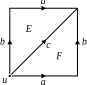
\includegraphics[width=0.4\columnwidth]{torus-delta.pdf}
	\caption[torus-delta]{$\Delta$-complex structure of a torus}
	\label{fig:torus-delta}
\end{figure}

The associated chain complex for taking simplicial homology is 
\begin{equation*}
	\begin{tikzcd}[row sep=tiny]
	\cdots & 0 & {E\Z \oplus F\Z} & {a\Z\oplus b\Z\oplus c\Z} & u\Z & 0 \\
	&&& {a,b,c} & 0 \\
	&& {E,F} & {a +b-c}
	\arrow["\partial_1", from=1-4, to=1-5]
	\arrow["\partial_2", from=1-3, to=1-4]
	\arrow[from=1-5, to=1-6]
	\arrow[from=1-2, to=1-3]
	\arrow[from=1-1, to=1-2]
	\arrow[maps to, from=3-3, to=3-4]
	\arrow[maps to, from=2-4, to=2-5]
\end{tikzcd}
\end{equation*}
Hence we get that
\begin{align*}
	H_0(\T^2) &\cong \Z,\\
	H_1(\T^2) &= \ker \partial_1 / \im \partial_2
	= a\Z \oplus b\Z \oplus c\Z / (a + b - c)\Z \cong \Z^2,\\
	H_2(\T^2) &= \ker \partial_2 = (E-F)\Z \cong \Z,
\end{align*}
and $H_n(\T^2) = 0$ for $n \geq 3$.
We deduce that the associated Betti numbers are
\begin{align*}
	b_0(\T^2) &= \rk(\Z) = 1,\\
	b_1(\T^2) &= \rk(\Z^2) = 2,\\
	b_2(\T^2) &= \rk(\Z) = 1,
\end{align*}
and $b_n(\T^2) = 0$ for $n \geq 3$.

\section{Elliptic Curves over Finite Fields}

\begin{definition}
	The zeta function of $V/\F_q$ is defined as the power series
	\begin{equation*}
		Z(V/\F_q; T) = \exp\left(\sum_{n=1}^\infty (\#V(\F_{q^n}))
		\frac{T^n}{n}\right)
	\end{equation*}
\end{definition}

\begin{notation}
	When $V/\F_q$ is known from context, we write simply $Z(T)$
	instead of $Z(V/\F_q; T)$
\end{notation}

\begin{theorem}[Weil Conjectures]
	Let $V/\F_q$ be a smooth projective variety of dimension $N$.
	\begin{enumerate}[label=(\alph*)]
		\item Rationality: $Z(T) \in \Q(T)$. More precisely, 
			there is a factorization
			\begin{equation*}
				Z(T) = \frac{P_1(T)\cdots P_{2n-1}(T)}
				{P_0(T)P_2(T) \cdots P_{2n}(T)},
			\end{equation*}
			where $P_0(T) = 1 - T, P_{2n}(T) = 1 - q^nT$ and for each
			$1 \leq i \leq 2n - 1$, $P_i(T)$ factors (over $\C$) as
			\begin{equation*}
				P_i(T) = \prod_j (1 - \alpha_{ij}T)
			\end{equation*}
		\item Functional Equation: The zeta function satisfies
			\begin{equation*}
				Z\left(\frac{1}{q^NT}\right) = \pm q^{N\frac{\epsilon}{2}}
				T^{\epsilon} Z(T),
			\end{equation*}
			for some integer $\epsilon$ (called the Euler characteristic of $V$)
		\item Riemann Hypothesis: $|\alpha_{ij}| = q^{i/2}$
			for all $1 \leq i \leq 2n - 1$ and all $j$.
		\item Betti Numbers: If $V/\F_q$ is a reduction mod $p$ of a
			non-singular projective variety $W/K$, where $K$ is a number
			field embedded in the field of complex numbers, then the degree
			of $P_i$ is the $i$\textsuperscript{th} Betti number of the space
			of complex points of $W$.
	\end{enumerate}
\end{theorem}

\begin{theorem}
	Let $E/\F_q$ be an elliptic curve. Then there exists an $a \in \Z$ such that
	\begin{equation*}
		Z(T) = \frac{1 - aT + qT^2}{(1-T)(1-qT)}.
	\end{equation*}
	Furthermore,
	\begin{equation*}
		Z\left(\frac{1}{qT}\right) = Z(T)
	\end{equation*}
	and
	\begin{equation*}
		1 - aT + qT^2 = (1 - \alpha T)(1 - \beta T)
	\end{equation*}
	with $|\alpha| = |\beta| = \sqrt{q}$
\end{theorem}

Hence the Weil conjectures are verified for elliptic curves. Notice that
$\deg P_0 = 1$, $\deg P_1 = 2$, $\deg P_2 = 1$, which coincides with the
Betti numbers we calculated in Section \ref{sec:over-C}.

\end{document}
